\section{Results}

\subsection{Comparison of the deregulated pathways in the PDCL with the TCGA-GBM datasets}

\subsubsection{Pathways mainly involved in the Cell-Cycle, DNA replication and Repair are shared between the two datasets}

The \acrshort{kegg} database document the processes affected in the case of many diseases including glioma.
Zyla \textit{et al} used the \textit{Glioma} entry (path:hsa05214) as a target pathway to assess the sensitivity of different ranking metrics when studying microarray data from brain tissue \cite*{Zyla2017}.
They used the p-value associated with the enriched pathway to assess the sensitivity of each method.
To recall, the p-value indicates how significantly enriched a pathway is, the lower the better.
Therefore, for the target result \textit{glioma}, the p-value should be very low when studying RNA-Seq data from glioblastoma.
We here use the \acrshort{fdr}, an adjusted p-value to correct for multiple hypothesis testing, to determine the sensitivity of G:Profiler and \acrshort{gsea} in our analysis.
Here, \acrshort{fdr} value for this pathway in G:Profiler is 0.008898 for \acrshort{pdcl} and 0.05240 for \acrshort{tcga}, in \acrshort{gsea} it is 0.004487 for \acrshort{pdcl} and 0.8298 for \acrshort{tcga}.
Not only the \acrshort{fdr} value is lower for the \acrshort{tcga} dataset but the \acrshort{fdr} of \acrshort{gsea} for \acrshort{pdcl} does not pass the threshold defined in this study.
Even if the \acrshort{fdr} value was below the threshold in G:Profiler for the \textit{Glioma} target result in \acrshort{pdcl}, because it was above the threshold for G:Profiler we do not consider this result enriched in the \acrshort{pdcl} dataset.
Controls for the \acrshort{pdcl} dataset are taken from another study \cite*{Lundin2018}, introducing experimental and biological variability independent from disease deregulation.
While controls in the \acrshort{tcga} dataset come from matching samples taken off the original tissue following the exact same protocol as the tumour samples to reduce such variability.
It might explain why \acrshort{gsea} failed to detect the \textit{Glioma} entry in the \acrshort{pdcl} dataset.

Like the \textit{Glioma} target result, we only consider a pathway to be enriched in a dataset if the \acrshort{fdr} value for this pathway is below the threshold in both G:Profiler and \acrshort{gsea}.
Thus, only the pathways that meet this criterion are presented and discussed in the results.
45 pathways are found deregulated in the \acrshort{pdcl} dataset and 304 in the \acrshort{tcga} dataset.
As can be seen in the figure \ref{fig:heatmap-fdr-global-tcga}, the two datasets shared 19 significantly deregulated pathways which are involved in the cell-cycle, DNA repair and replication, gene expression, extracellular matrix and diseases.
\begin{figure}
    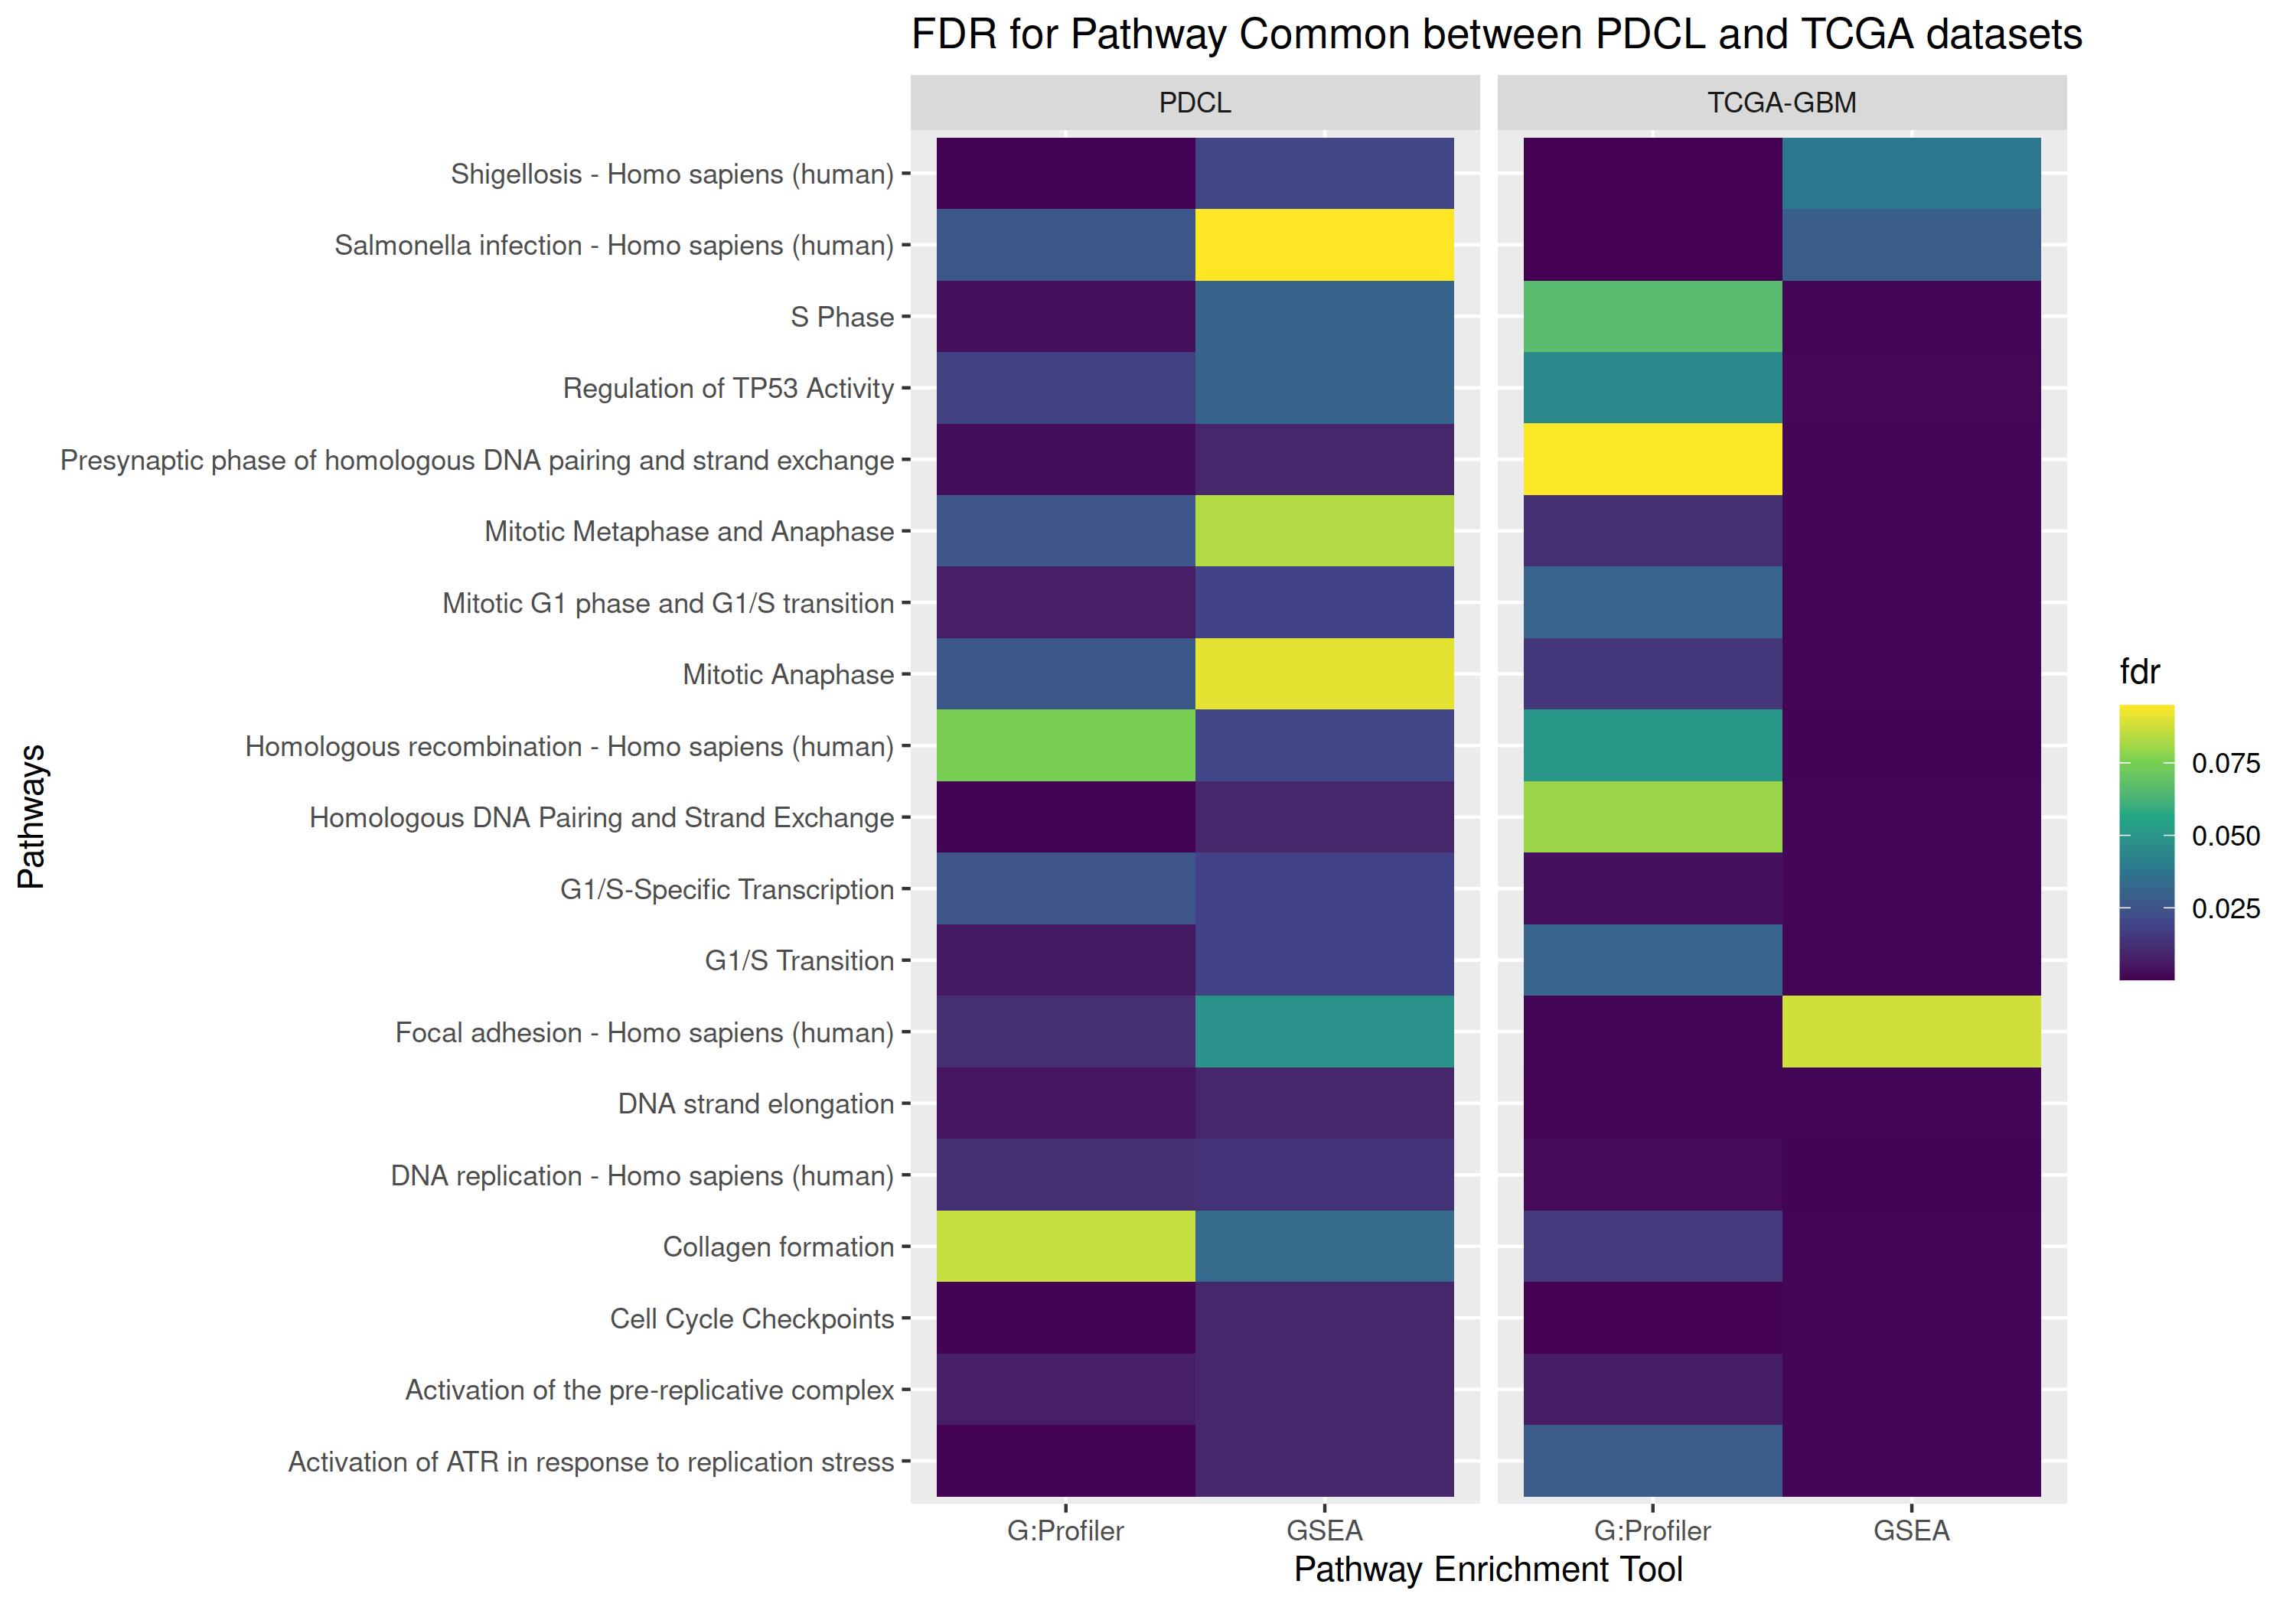
\includegraphics[width=\textwidth]{img/heatmap-fdr-global-tcga}
    \caption{
        \acrfull{fdr} of the pathways deregulated in both the \acrshort{pdcl} and the \acrshort{tcga} datasets.
        \acrshort{fdr} is lower than 0.1 since we only keep pathways below this value.
    }
    \label{fig:heatmap-fdr-global-tcga}
\end{figure}
The 2 pathways associated with disease (Shigellosis and Salmonella infection) belong to the \acrshort{kegg} database.
However, pathways involved in DNA replication and repair are significantly enriched for both \acrshort{kegg} and Reactome.
Interestingly, \textit{Regulation of TP53 activity} is found upregulated by \acrshort{gsea} for both datasets.
A study from \acrshort{tcga} on frequent mutations in glioblastoma has shown that p53 signalling is altered in 87\% of the samples and p53 is inactivated by mutation in 35\% of the samples \cite*{McLendon2008}.
Thus, the regulation of p53 may be upregulated to make up for the lack of activity from the mutated p53.

As can be seen in the figure \ref*{fig:complete-piechart-categ-pdcl}, the most deregulated category in the \acrshort{tcga} dataset is the \textit{Organismal Systems} category which includes biological processes involved in the Immune system, Endocrine system, Circulatory system, Digestive system, Sensory system, etc.
In the \acrshort{pdcl} dataset, \textit{Cell Cycle} is the most deregulated category in both the global and the personalized analysis (the analysis where each \acrshort{pdcl} samples are compared one by one to all the controls, lower panel in figure \ref*{fig:workflow-diagram-global}).
The \textit{Signal Transduction}, \textit{Metabolism of RNA and proteins} and the \textit{Cell-Cycle} categories are among the top 5 most deregulated categories in \acrshort{tcga}.
In comparison, less categories are affected in the global analysis for the \acrshort{pdcl} dataset, with \textit{DNA Processes} and \textit{Cell-Cycle} categories among the top 3 most deregulated categories.
In both \acrshort{tcga} and the global analysis of \acrshort{pdcl}, the \textit{Disease} category is the second most affected category.
\begin{figure}
    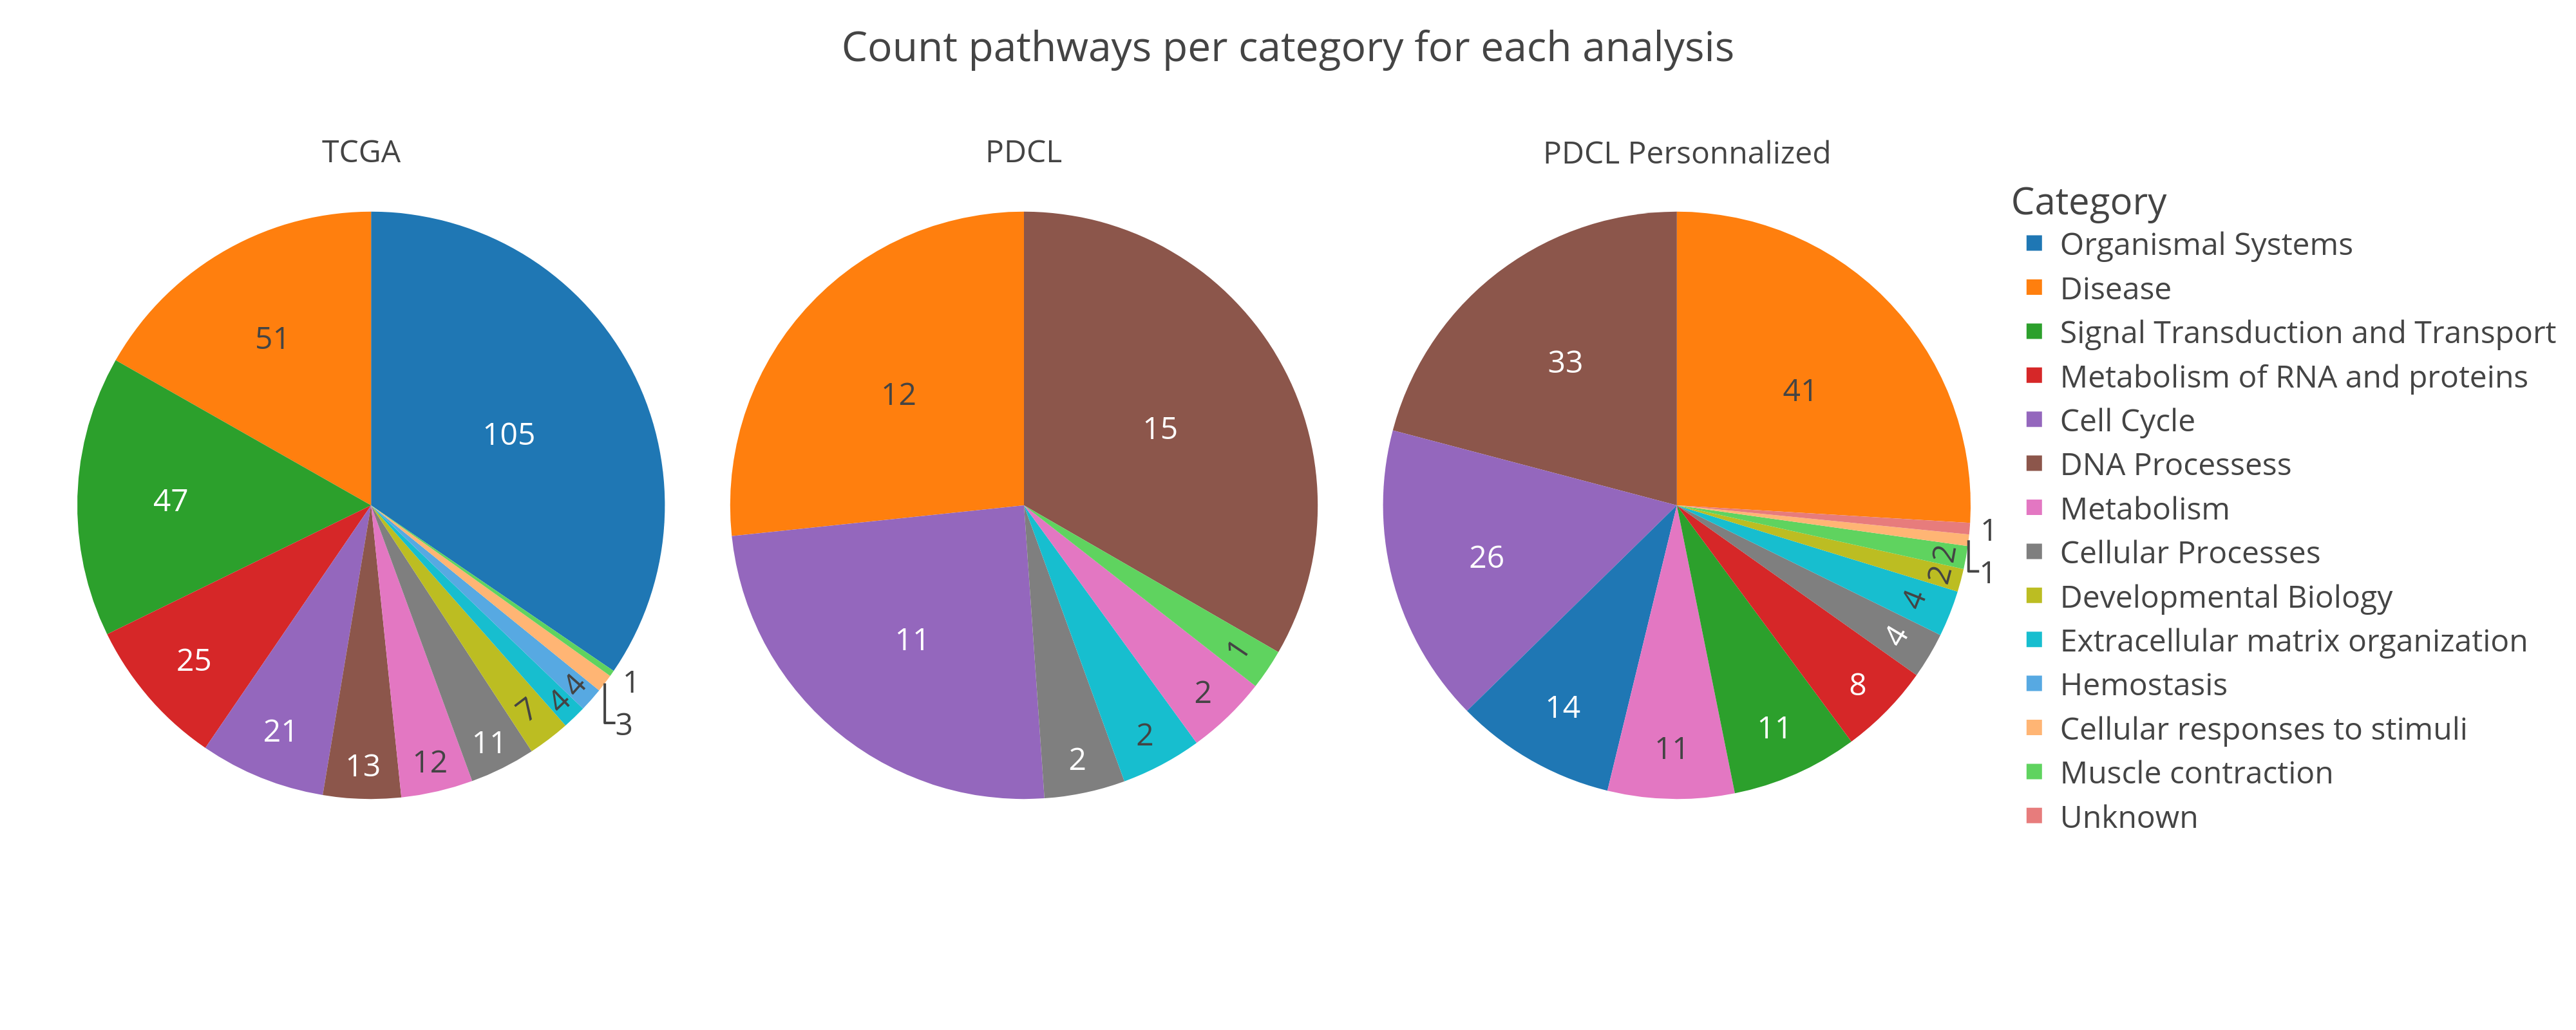
\includegraphics[width=\textwidth]{img/complete-piechart-categ-pdcl}
    \caption{
        Number of deregulated pathways per category and per analysis.
        The results are presented for the \acrshort{tcga} dataset, the global analysis and the personalized analysis of the \acrshort{pdcl} dataset.
        To recall, during the personalized analysis with compared each \acrshort{pdcl} samples against all the controls one by one (lower panel in figure \ref*{fig:workflow-diagram-global}).
        In the personalized analysis of the \acrshort{pdcl} dataset, only different results can contribute to the number of pathways for a category.
        Thus, a same pathway that is found deregulated in two different samples will only be counted once.
        The \textit{Organismal Systems} category includes pathways involved in the Immune system, Endocrine system, Circulatory system, Digestive system, Sensory system, etc.
        Among all analysis, the \textit{Disease} category is the first or the second most deregulated category.
        For \acrshort{tcga}, the top 5 most deregulated categories includes \textit{Organismal Systems}, \textit{Signal Transduction and Transport}, \textit{Metabolism of RNA and proteins} and \textit{Cell-Cycle}.
        While for the \acrshort{pdcl} dataset (global analysis), the most deregulated categories include \textit{Cell-Cycle} and \textit{DNA processeses}.
        The deregulated pathways in the personalized analysis of the \acrshort{pdcl} dataset mostly belong to the \textit{Cell-Cycle}, \textit{DNA processeses} and \textit{Organismal Systems}, \textit{Metabolism} and \textit{Signal Transduction and Transport}.
    }
    \label{fig:complete-piechart-categ-pdcl}
\end{figure}

\subsubsection{Cell-Cycle}

Two phases of the Cell Cyle are enriched in both datasets : the \textit{S phase} (R-HSA-69242) and the \textit{Mitotic Anaphase} (R-HSA-68882).
Interestingly, when in a first intention we kept pathways between 15 and 1,000 genes, \textit{Mitotic Anaphase}  was enriched only in \acrshort{tcga}.
It was enriched as well in the \acrshort{pdcl} dataset after we set up the boundary between 15 to 500 genes.
It highlights that the number of pathways present in the \acrshort{gmt} file has an impact on the significance of the results.

For both dataset, the textit{Cell Cycle Checkpoints} pathway (R-HSA-69620) is affected.
Other pathways linked to the S phase of the cell-cycle are shared between datasets such as the \textit{DNA strand elongation} (R-HSA-69190) taking place in the S phase and the \textit{G1/S-Specific Transcription} (R-HSA-69205).

Among the pathways enriched only in the \acrshort{tcga} dataset, we found pathways that are children of pathways shared between both datasets.
For example, \textit{Amplification of signal from unattached kinetochores via a MAD2 inhibitory signal} (R-HSA-141444) is a children pathway of \textit{Cell Cycle Checkpoints} (R-HSA-69620), that is to say it is smaller pathway which takes place in its parent pathways.
Only G:Profiler's result for this pathway in the \acrshort{pdcl} dataset does not pass the threshold (\acrshort{fdr} is equal to 0.125).
We first hypothesized that the lower number of genes included in the \acrshort{pdcl} dataset (~20,000 genes compared to ~60,000 in \acrshort{tcga}) may be the cause.
Nonetheless, almost all the genes involved in this pathway are present in the \acrshort{pdcl} dataset.
A closer look at the number of genes that are deregulated and involved in this pathway shows 74 genes for \acrshort{tcga} compared to 48 for \acrshort{pdcl}, indicating that the number of deregulated genes is more likely to be at cause here.
This example may explain why other children processes taking place in a larger function are not detected in \acrshort{pdcl} compared to \acrshort{tcga} but may be affected.

\subsubsection{Metabolism}

Although pathways involved in metabolism are enriched in both datasets, none of them are shared between the two datasets.
The \acrshort{tcga} dataset is mostly enriched with pathways involved in the energetic metabolism such as \textit{Phospholipid metabolism} (R-HSA-1483257), \textit{Regulation of insuline secretion} (R-HSA-422356) and \textit{Selenoamino acid metabolism} (R-HSA-2408522).
The glycerophospholipid metabolism, part of phospholipid metabolism, is enriched in both Reactome and \acrshort{kegg} database.
The \acrshort{tcga} dataset is also enriched with pathways involved in the Metabolism of proteins or the Metabolism of RNA such as \textit{Peptide chain elongation} (R-HSA-156902), \textit{Translation initiation complex formation} (R-HSA-72649) and \textit{rRNA processing in the nucleus and cytosol} (R-HSA-8868773).

Compared to the \acrshort{tcga} dataset, there are no pathways involved in the Metabolism of proteins or the Metabolism of RNA enriched in the \acrshort{pdcl}.
The only pathway involved in metabolism found deregulated is the \textit{Cholesterol Biosynthesis} (R-HSA-191273) and the \textit{Steroid biosynthesis} (path:hsa00100), 2 pathways having a role in cholesterol metabolism.

\subsubsection{Extra-Cellular Matrix}

The \textit{Collagen formation} (R-HSA-1474290) and \textit{focal adhesion} (path:hsa04510) pathways are shared between the \acrshort{tcga} and \acrshort{pdcl} datasets.
They are related to the \acrlong{ecm} and the cell-matrix interactions as collagen is a protein composing the \acrshort{ecm} and the \textit{focal adhesion} is a process where the cell adheres to the matrix.
Only in the \acrshort{tcga} dataset, the \textit{Assembly of collagen fibrils and other multimeric structures} (R-HSA-2022090) and the \textit{Collagen biosynthesis and modifying enzymes} (R-HSA-1650814), two pathways included in the \textit{Collagen formation}, are found enriched.
The \textit{\acrshort{ecm}-receptor interaction} (path:hsa04512), \textit{Cell adhesion molecules} (path:hsa04514) and the \textit{Laminin interaction} (R-HSA-3000157) are pathways related to the adhesion of the cell to the \acrshort{ecm} only enriched in the \acrshort{tcga} datasets as well.
The \textit{Non-integrin membrane-ECM interactions} (R-HSA-3000171) is another pathway related to the \acrshort{ecm}-cell interactions yet only found enriched in the \acrshort{pdcl}.
The results seem to indicate that \acrshort{ecm} and cell adhesion carry a role in glioblastoma growth.
Since the \textit{Collagen formation} pathway is shared by the two datasets, it suggests that this process is important for glioblastoma growth.
However, \textit{Laminin interaction} and \textit{Non-integrin membrane-ECM interactions}, two pathways classified on the same level in the hierarchy of Reactome, tend to show different mechanisms by which the tumour cell can influence its adhesion to the \acrshort{ecm}.
Surprisingly, \textit{Focal adhesion} and \textit{Collagen formation} were both upregulated in \acrshort{tcga} but downregulated in \acrshort{pdcl}.
This may be due to the controls used in the \acrshort{pdcl} dataset.

\subsection{Comparison of the deregulated pathways between PDCLs}

\subsubsection{Cell adhesion to the ECM is the most frequently deregulated pathway}

Table \ref*{table:frequently-dereg-pathways} shows the pathways found deregulated in at least 3 different \acrshort{pdcl} samples.
\textit{Focal adhesion}, a pathway previously found deregulated in \acrshort{tcga} and \acrshort{pdcl}, is the most commonly deregulated pathway with 13 different samples out of 20.
Hence, this pathway might be important for glioblastoma progression.
Corroborating this hypothesis, other pathways involved in collagen synthesis and interactions \acrshort{ecm}-cell interactions are deregulated in 3 to 6 different samples (R-HSA-1650814, path:hsa04512, R-HSA-8948216, R-HSA-1474290).

In a similar way, \textit{Steroid biosynthesis} and \textit{Cholesterol biosynthesis}, two pathways identified in the \acrshort{pdcl} during the global analysis, are found deregulated in 5 and 3 different samples, respectively.
Despite it is not found enriched in the global analysis, the \textit{Oxidative phosphorylation} (path:hsa00190), well-known for its role in the generation of \acrshort{atp}, is found deregulated in 5 samples.
This pathway has been widely studied due to its important role in the generation of \acrshort{atp} and its potential implication in the Warburg Effect, an increase of usage of glycolysis to produce \acrshort{atp} even though oxygen is available \cite*{Spinicci2022}.
It was first hypothesized that mitochondria were defective in tumour cells, yet it was later mitochondrial function was similar to normal cells \cite*{Cairns2011}.
Since this pathway is upregulated in 5 different samples but not detected in the global analysis, it might be cell-dependant rather than a feature of bulk tumours.
The second most frequently deregulated pathway is the \textit{Axon guidance} (path:hsa04360), a pathway involved in the formation of the neuronal network using guidance factors to influence the way the growth cone will turn.
The \textit{Hippo signaling pathway} (path:hsa04392, path:hsa04390) and \textit{Retrograde endocannnabinoid signaling} (path:hsa04723), two signaling pathway whose role in cancer have been documented in the litterature, are found deregulated in 6 and 5 different samples, respectively.
\todo{read the article about them before citing them as references}

\begin{table}
    \centering
    \resizebox*{\textwidth}{!}{
        \begin{tabular}{ |c|c|c|c|c| }
            \hline
            Pathway ID & Description & Database & Category & Number of PDCL \\
            \hline
            path:hsa04510 & Focal adhesion & KEGG & Cellular Processes & 13 \\
            path:hsa04360 & Axon guidance & KEGG & Organismal Systems & 9 \\
            R-HSA-1650814 & Collagen biosynthesis and modifying enzymes & Reactome & ECM & 6 \\
            path:hsa00100 & Steroid biosynthesis & KEGG & Metabolism & 5 \\
            path:hsa00190 & Oxidative phosphorylation & KEGG & Metabolism & 5 \\
            path:hsa04392 & Hippo signaling pathway - multiple species & KEGG & Environmental Information Processing & 5 \\
            path:hsa04512 & ECM-receptor interaction & KEGG & Environmental Information Processing & 5 \\
            path:hsa04723 & Retrograde endocannabinoid signaling & KEGG & Organismal Systems & 5 \\
            R-HSA-8948216 & Collagen chain trimerization & Reactome & ECM & 5 \\
            path:hsa03008 & Ribosome biogenesis in eukaryotes & KEGG & Genetic Information Processing & 3 \\
            path:hsa03020 & RNA polymerase & KEGG & Genetic Information Processing & 3 \\
            path:hsa04390 & Hippo signaling pathway & KEGG & Environmental Information Processing & 3 \\
            path:hsa04612 & Antigen processing and presentation & KEGG & Organismal Systems & 3 \\
            path:hsa04714 & Thermogenesis & KEGG & Organismal Systems & 3 \\
            R-HSA-1474290 & Collagen formation & Reactome & ECM & 3 \\
            R-HSA-176187 & Activation of ATR in response to replication stress & Reactome & Cell Cycle & 3 \\
            R-HSA-191273 & Cholesterol biosynthesis & Reactome & Metabolism & 3 \\
            R-HSA-5693538 & Homology Directed Repair & Reactome & DNA Repair & 3 \\
            R-HSA-6790901 & rRNA modification in the nucleus and cytosol & Reactome & Metabolism of RNA & 3 \\
            \hline
        \end{tabular}
    }
    \caption{
        Table of the frequently deregulated pathways in the \acrshort{pdcl} dataset when assessing the alteration specific to each sample.
        The table includes only pathways deregulated in at least three different samples which account for 18 pathways.
        The most frequently deregulated pathway is the \textit{Focal adhesion} (slightly more than half of the samples) which is also found deregulated in \acrshort{tcga}.
        The \acrshort{kegg} database include two different entries for the \textit{Hippo signaling} pathway.
        Taken together, the \textit{Hippo signalling} pathway is found deregulated in 6 samples.
    }
    \label{table:frequently-dereg-pathways}
\end{table}

\subsubsection{Differencies in deregulated processes between PDCL samples}

In the global analysis of the \acrshort{pdcl} dataset, only two deregulated pathways are associated with the \textit{Metabolism} and none with the \textit{Metabolism of RNA and proteins} and \textit{Signal Transduction and Transport} (figure \ref*{fig:complete-piechart-categ-pdcl}).
In contrast, the personnalized analysis of this dataset shows eleven deregulated pathways in \textit{Metabolism} and \textit{Signal Transduction and Transport}, and eight in \textit{Metabolism of RNA and proteins}.
This seems to indicate that \textit{Metabolism}, \textit{Metabolism of RNA and proteins} and \textit{Signal Transduction and Transport} are biological categories with high heterogeneity in the \acrshort{pdcl} dataset.

\begin{figure}
    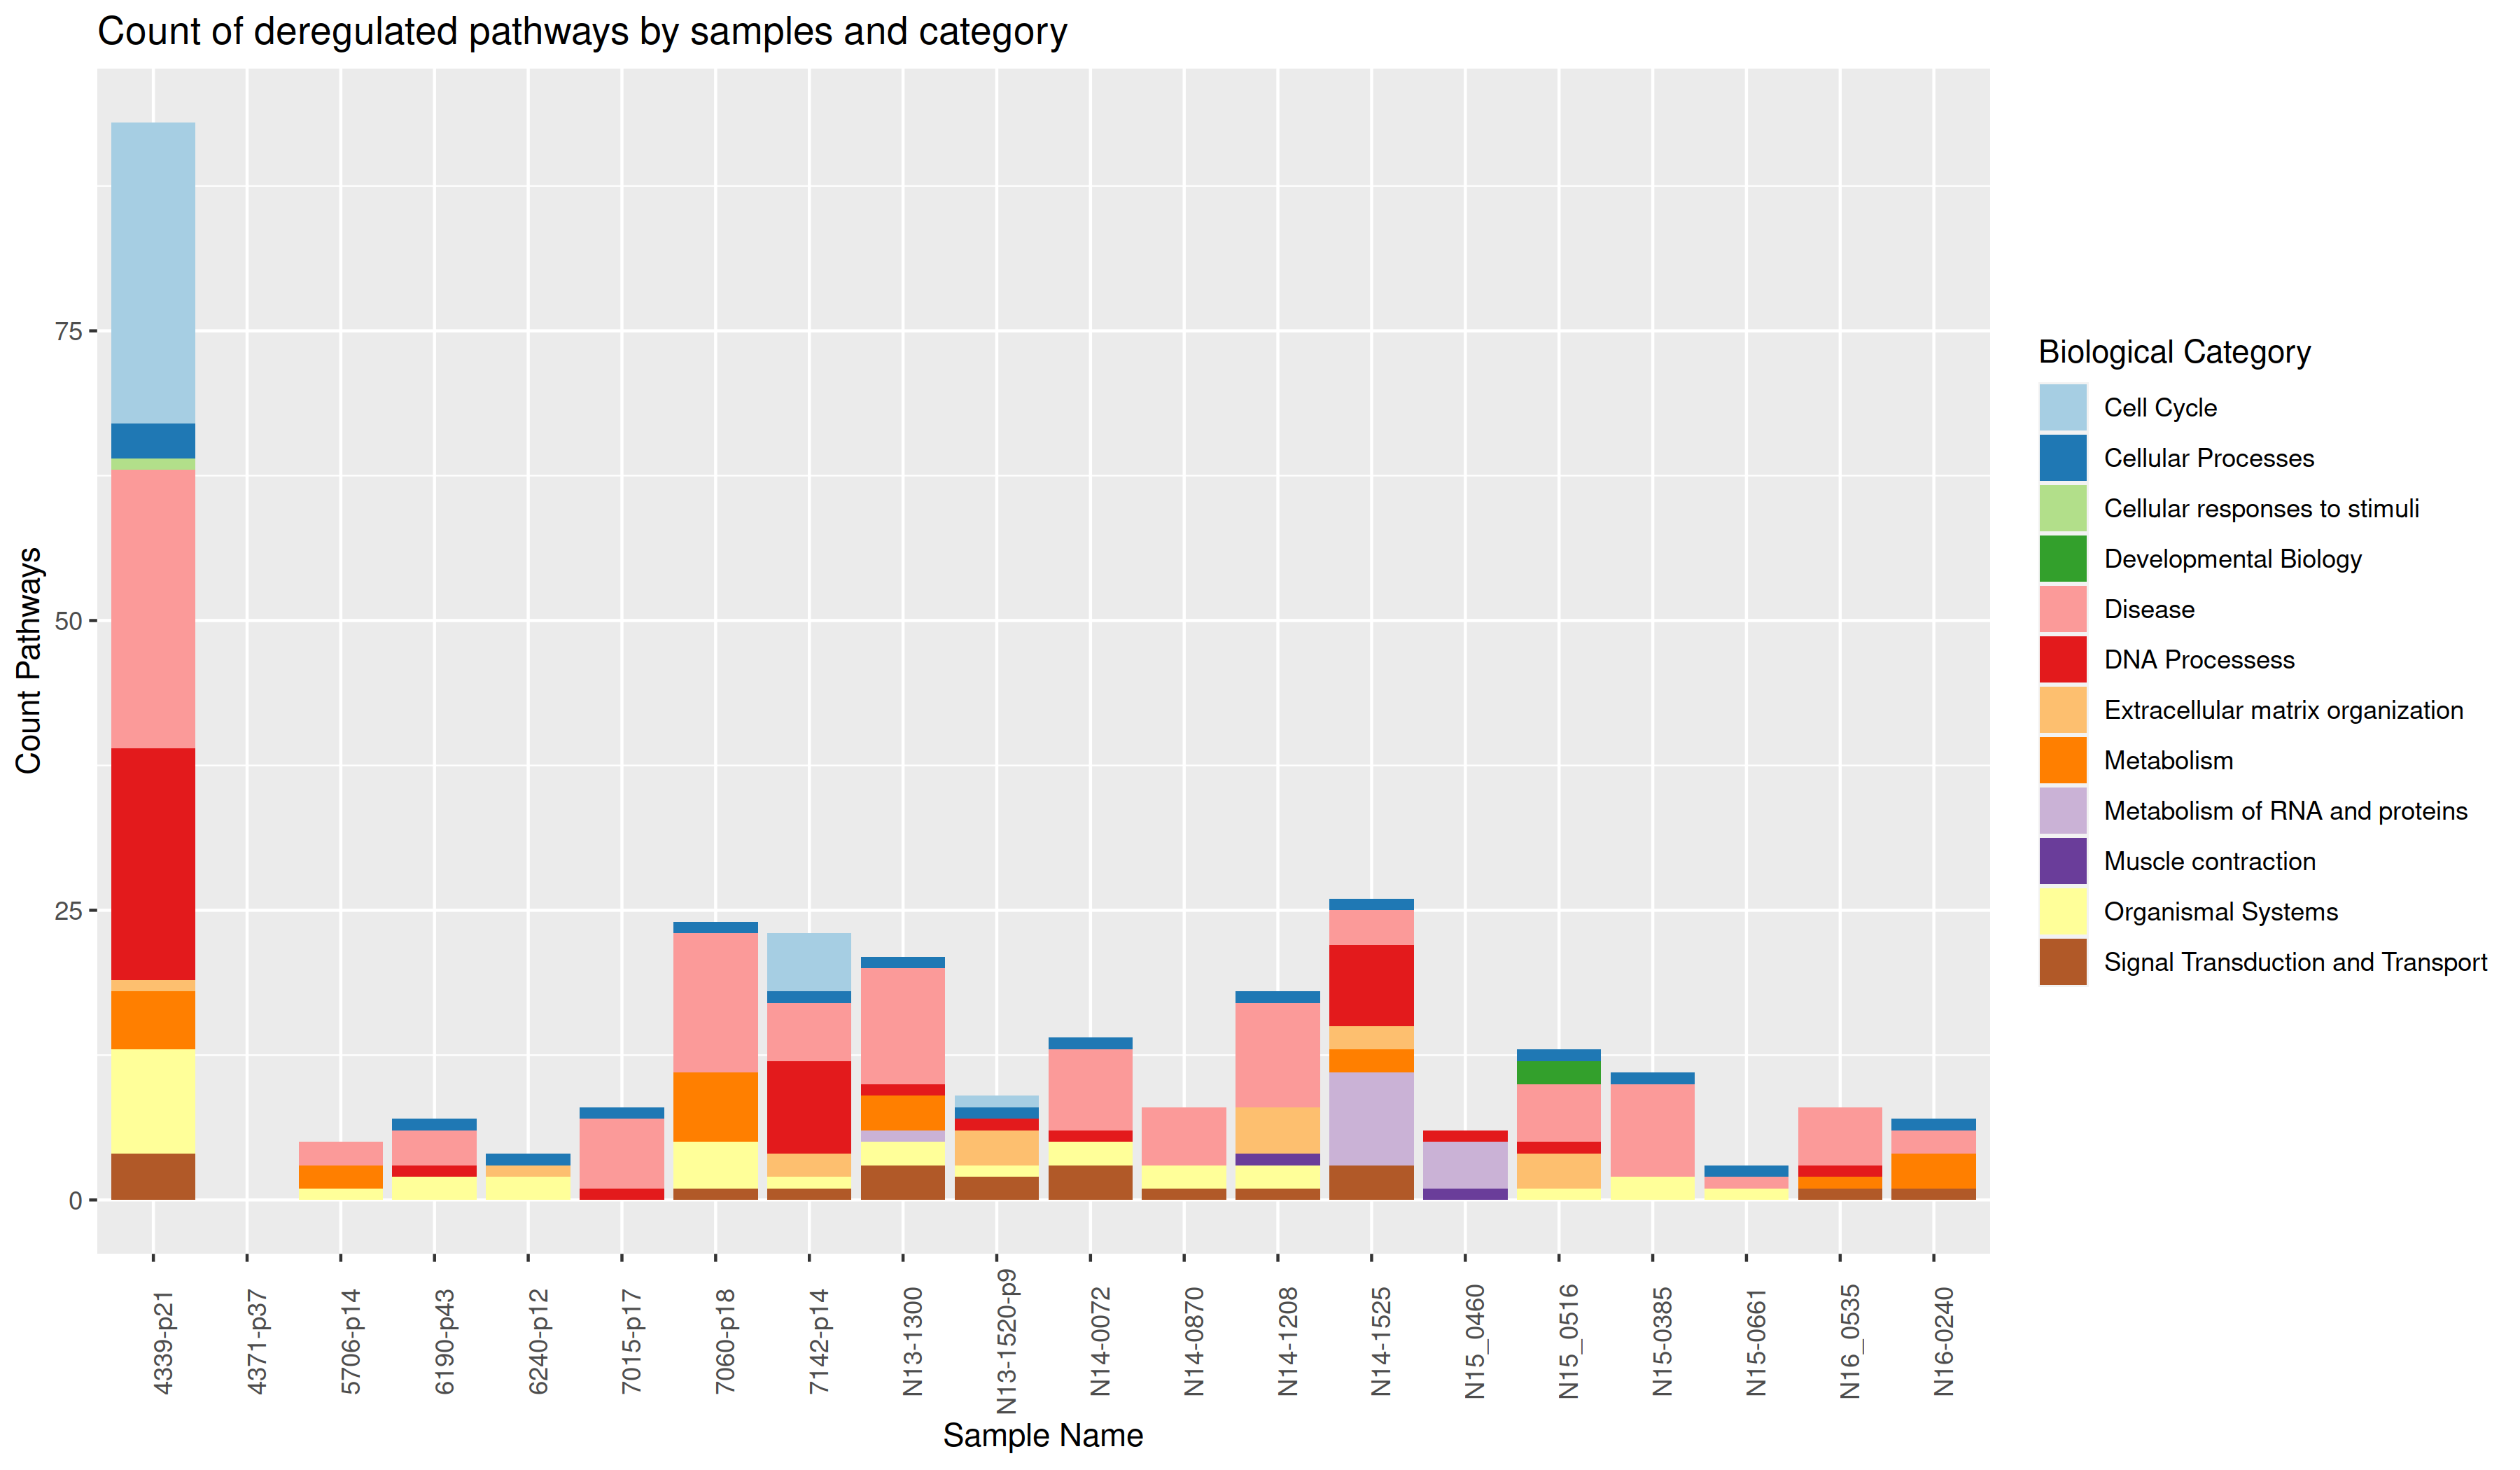
\includegraphics[width=\textwidth]{img/barplot-categ-pdcl}
    \caption{
        Number of deregulated pathways per category and per sample in \acrshort{pdcl} datasets.
        Among the samples, the categories frequently affected are involved in Disease, DNA Processesses, Organismal System and Signal Transduction/Transport.
        Sample 4339-p21 is the \acrshort{pdcl} with the biggest number of deregulated pathways, they are mainly involved in the Cell-Cycle or DNA processes (DNA repair and replication).
        No pathways pass the significance threshold in G:Profiler and \acrshort{gsea} at the same time for the samples 4371-p37.
        The \acrshort{kegg} entry \textit{Biosynthesis of cofactors} (path:hsa01240) is enriched in the sample 4339-p21 but it could not be mapped to a biological category, we remove it from the plot to simplify visualization. 
    }
    \label{fig:barplot-categ-pdcl}
\end{figure}

Even though that pathways were below the significance threshold in G:Profiler and \acrshort{gsea}, one sample of the \acrshort{pdcl} dataset (4371-p37) has no pathways common to both enrichment methods and thus has no pathways found deregulated.
As can be seen in figure \ref*{fig:barplot-categ-pdcl}, the pathways deregulated in the sample 4339-p21 are mainly involved in the Cell-Cycle or DNA processes (DNA repair and replication).
Not only it is the sample with the most deregulated pathways, but it is the sample with the most biological processes taking place in cell cycling affected as well.

\begin{figure}
    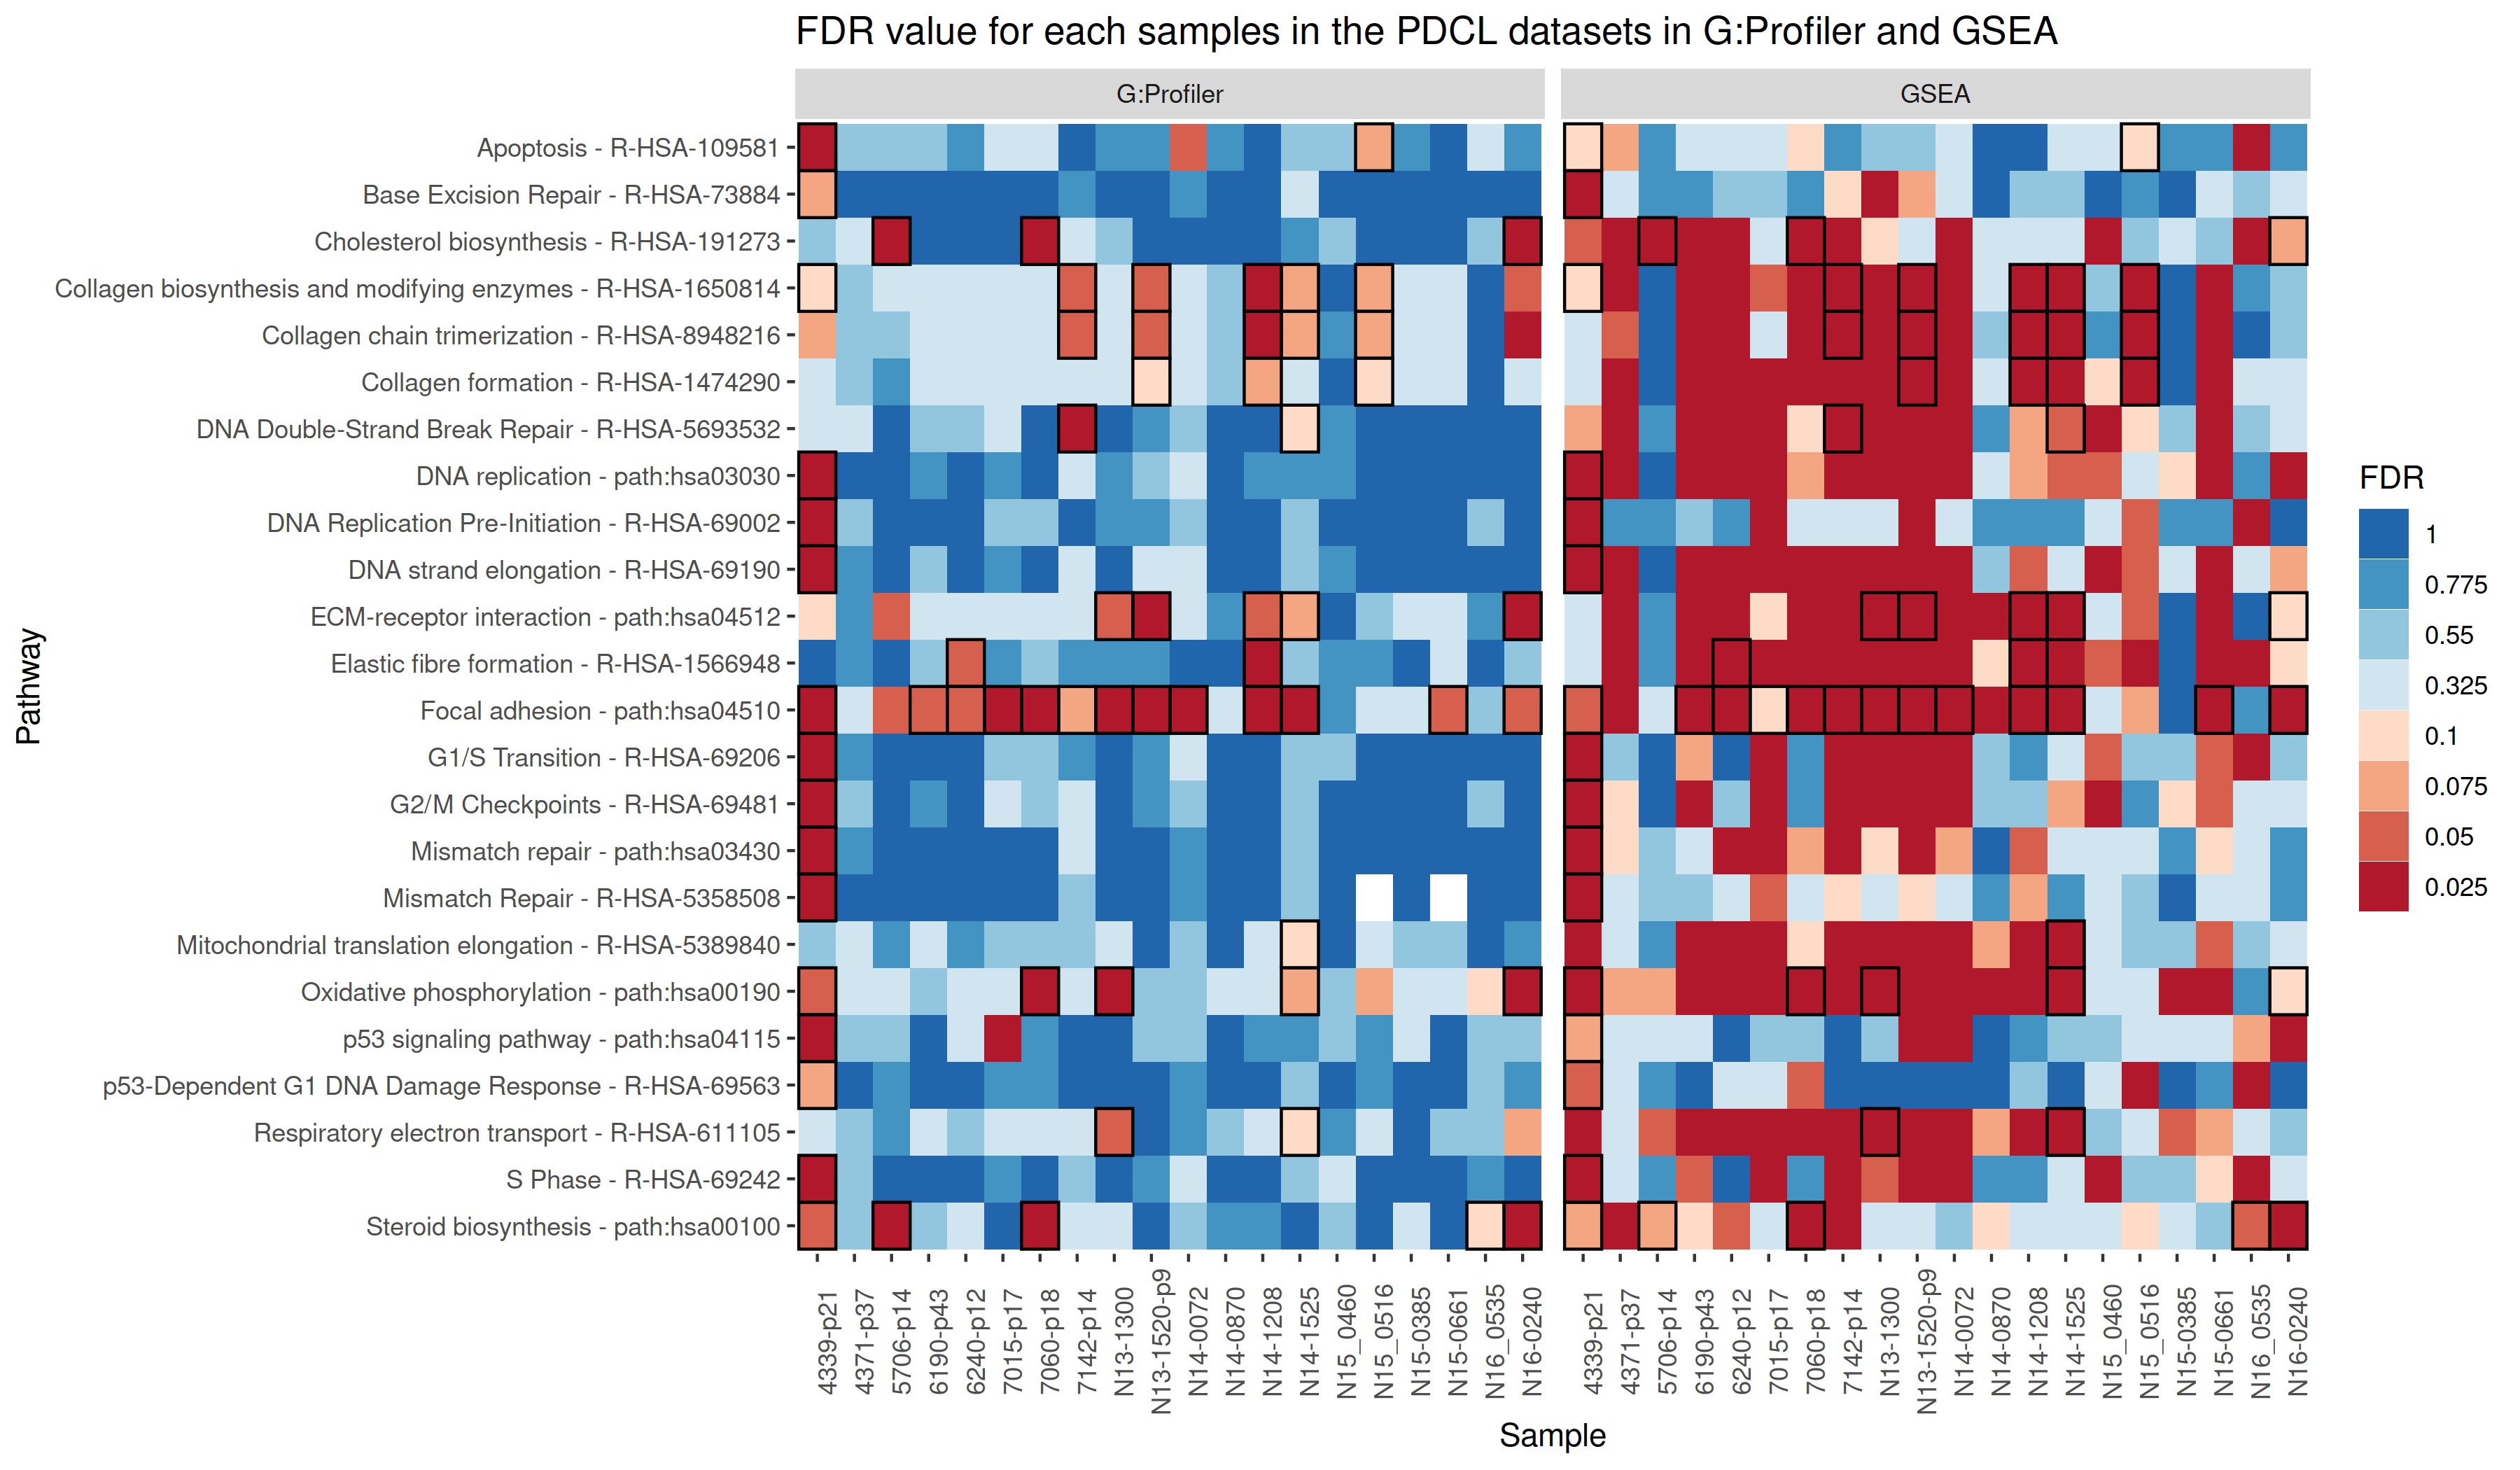
\includegraphics[width=\textwidth]{img/heatmap-fdr-pathway}
    \caption{
        G:Profiler and \acrshort{gsea} \acrfull{fdr} of the pathways deregulated for each samples in the \acrshort{pdcl} datasets.
        Pathways below the significance threshold in both pathway enrichment tools are highlighted in a black box.
        Pathways were manually selected to avoid redundancy of the informations, overloading the plot with numerous entry and show processes with ease of Interpretation.
        We kept pathways that were not tooo general because they do not bring meaningfull information, nor pathways that were too precise since they are difficult to link to more known processes.        
        Deregulated pathways are mostly involved in the Cell-Cycle, DNA repair, \acrlong{ecm} and Metabolism.
    }
    \label{fig:heatmap-fdr-pathway}
\end{figure}

Figure \ref*{fig:heatmap-fdr-pathway} shows that the part of the cell cycle affected for the sample 4339-p21 are the G1/S phases transition, checkpoints in G1 and G2/M phase, DNA repair system and p53 signalling.
p53 is one of the most frequently mutated genes in the case of glioblastoma \cite*{McLendon2008}.
7142-p14 and N14-1525 shows also dysregulation of the \textit{DNA Double-Strand Break Repair} system, despite none of the pathways involved in the different phases of the Cell Cycle are affected.
Samples N13-1300 and N14-1525 are the only samples with a dysregulation in the \textit{Oxidative Phosphorylation} that also present alterations in the \textit{Respiratory electron transport}, N14-1525 showing in addition alteration of the \textit{Mitochondrial translation}.
